\chapter{Exemples LaTeX courants}
\label{app:latex-patterns}

% Cette annexe facultative est un aide-mémoire et ne fait pas partie de
% l'argument sur l'accessibilité. Ne conservez que les formes réellement
% utilisées, remplacez chaque ressource pédagogique et commentez dans le texte
% toute figure, tout tableau, toute équation ou tout extrait de code conservé.

\section{Illustration externe}

Le projet contient le fichier vectoriel original utilisé dans
la \cref{fig:external-illustration}. L'extension \texttt{.pdf} explicite indique
qu'il s'agit d'une ressource externe chargée avec \verb|\includegraphics|, et
non de code TikZ inséré avec \verb|\input|. Le format PDF convient aux schémas
et graphiques ; PNG ou JPEG convient à une image véritablement matricielle.

\begin{figure}[htbp]
  \centering
  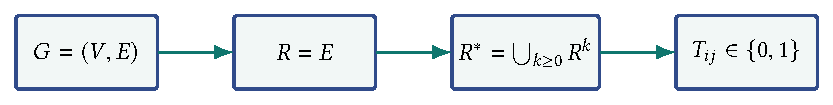
\includegraphics[width=0.82\linewidth]{figures/example-workflow.pdf}
  \caption{Illustration PDF externe et originale du déroulement de l'exemple.}
  \label{fig:external-illustration}
\end{figure}

% Remplacez le fichier et la légende. Indiquez la source et la licence de
% toute image non originale, ne déformez pas une image en imposant des
% dimensions incompatibles et contrôlez sa lisibilité à la taille
% d'impression.

\section{Équations multilignes et définition par cas}

Utilisez \texttt{align} lorsque plusieurs lignes constituent une même dérivation
et s'alignent sur un symbole pertinent. Étiquetez uniquement les lignes citées
ensuite. Par exemple,
\begin{align}
  T^{(0)}_{ij}
    &= A_{ij}\lor [i=j], \label{eq:pattern-initialisation}\\
  T^{(k)}_{ij}
    &= T^{(k-1)}_{ij}
       \lor\bigl(T^{(k-1)}_{ik}\land T^{(k-1)}_{kj}\bigr).
       \label{eq:pattern-update}
\end{align}
La mise à jour de l'\cref{eq:pattern-update} ajoute les chemins dont le nouveau
sommet intermédiaire autorisé est $k$.

Une définition par cas appartient à une équation numérotée lorsqu'elle doit être
citée :
\begin{equation}
  d(u,v)=
  \begin{cases}
    0, & u=v,\\
    \text{longueur d'un plus court chemin}, & v\text{ est accessible depuis }u,\\
    +\infty, & \text{sinon}.
  \end{cases}
  \label{eq:pattern-cases}
\end{equation}

\section{Tableau avec texte long}

Les colonnes \texttt{X} du \cref{tab:pattern-guide} partagent la largeur
disponible et renvoient automatiquement le texte à la ligne. Préférez
\texttt{tabular} pour des données numériques compactes et n'introduisez
\texttt{longtable} que si un véritable tableau doit se poursuivre sur plusieurs
pages, comme ci-dessous.

\begin{table}[htbp]
  \centering
  \caption{Choix d'une forme de tableau compacte.}
  \label{tab:pattern-guide}
  \begin{tabularx}{\linewidth}{@{}l>{\raggedright\arraybackslash}X>{\raggedright\arraybackslash}X@{}}
    \toprule
    Contenu & Traitement recommandé & Erreur fréquente \\
    \midrule
    Mesures & Indiquer unités et incertitude dans l'en-tête ou une note. & Répéter l'unité dans chaque cellule. \\
    Descriptions longues & Utiliser une colonne \texttt{X} et un texte concis. & Réduire tout le tableau jusqu'à rendre le texte illisible. \\
    Nombreuses lignes & Envisager une annexe ou un fichier lisible par machine. & Découper manuellement une ligne logique entre deux pages. \\
    \bottomrule
  \end{tabularx}
\end{table}

\section{Tableau sur plusieurs pages}

\texttt{longtable} permet à un même tableau logique de se poursuivre sur
plusieurs pages. La légende et les en-têtes de colonnes sont déclarés une seule
fois, et le bloc d'en-tête est répété sur chaque page suivante.
Le \cref{tab:pattern-checklist} montre ce schéma avec une liste de contrôle avant
dépôt.

\begin{longtable}{@{}p{0.2\linewidth}p{0.62\linewidth}c@{}}
  \caption{Liste de contrôle composée avec \texttt{longtable}.}
  \label{tab:pattern-checklist}\\
  \toprule
  Domaine & Point à vérifier & Fait \\
  \midrule
  \endfirsthead
  \toprule
  Domaine & Point à vérifier & Fait \\
  \midrule
  \endhead
  \midrule
  \multicolumn{3}{r@{}}{\emph{Suite page suivante}}\\
  \endfoot
  \bottomrule
  \endlastfoot
  Métadonnées & Titres, auteur, encadrants, année universitaire, date et mots-clés sont corrects. & $\square$ \\
  Langue & Le document principal choisi et la langue des métadonnées PDF concordent. & $\square$ \\
  Commentaires & Les commentaires de conseil (lignes commençant par \texttt{\%}) ne décrivent plus l'exemple. & $\square$ \\
  Couverture & Logos, encadrants, enseignant référent et laboratoire sont corrects et autorisés. & $\square$ \\
  Résumé & Le résumé énonce la question, la méthode, le résultat principal et les limites. & $\square$ \\
  Sommaire & Chaque chapitre et chaque annexe apparaît avec le bon numéro de page. & $\square$ \\
  Chapitres & Les chapitres d'exemple sont remplacés et aucun fichier inutile n'est inclus. & $\square$ \\
  Figures & Chaque figure est citée, légendée en dessous et lisible à l'impression. & $\square$ \\
  Tableaux & Chaque tableau est cité et légendé au-dessus, avec ses unités. & $\square$ \\
  Équations & Seules les équations citées plus loin portent une étiquette. & $\square$ \\
  Théorèmes & Les énoncés sont numérotés par chapitre et chacun est utilisé ou commenté. & $\square$ \\
  Bibliographie & Toute entrée imprimée est citée ; DOI et années ont été vérifiés. & $\square$ \\
  Liens & Renvois et citations sont résolus et aucun renvoi ne reste indéfini. & $\square$ \\
  Compilation & Une compilation complète propre ne signale ni fichier manquant ni boîte trop large. & $\square$ \\
  PDF & Les polices sont incorporées et chaque page a été relue. & $\square$ \\
  Dépôt & Le PDF final respecte les consignes du programme et de l'encadrement. & $\square$ \\
\end{longtable}

% Remplacez les lignes par votre propre tableau. Placez la légende au-dessus
% du tableau, gardez des structures de colonnes identiques pour \endfirsthead
% et \endhead, et évitez longtable pour un tableau qui tient confortablement
% sur une page.

\clearpage
\section{Code source}

Le paquet portable \texttt{listings} utilisé dans l'\cref{lst:graph-traversal}
ne demande pas de shell escape ; la coloration reste volontairement discrète.

% Pour un long programme, placez-le dans son propre fichier et chargez-le avec
% \lstinputlisting[style=TemplateCode,language=Python]{code/mon-programme.py}
\begin{lstlisting}[
  style=TemplateCode,
  language=Python,
  caption={Un court parcours de graphe.},
  label={lst:graph-traversal}
]
def reachable(graph, source):
    seen = {source}
    frontier = [source]
    while frontier:
        vertex = frontier.pop()
        for neighbor in graph.get(vertex, []):
            if neighbor not in seen:
                seen.add(neighbor)
                frontier.append(neighbor)
    return seen
\end{lstlisting}

Ensemble, ces quatre exemples
(\cref{fig:external-illustration,eq:pattern-cases,tab:pattern-guide,lst:graph-traversal})
illustrent le cycle recommandé : annoncer un objet, le présenter, lui attribuer
une étiquette stable et l'interpréter dans le texte.
